% Тут используется класс, установленный на сервере Papeeria. На случай, если
% текст понадобится редактировать где-то в другом месте, рядом лежит файл matmex-diploma-custom.cls
% который в момент своего создания был идентичен классу, установленному на сервере.
% Для того, чтобы им воспользоваться, замените matmex-diploma на matmex-diploma-custom
% Если вы работаете исключительно в Papeeria то мы настоятельно рекомендуем пользоваться
% классом matmex-diploma, поскольку он будет автоматически обновляться по мере внесения корректив
%

\title{Генератор абстрактных лексических анализаторов}
%
\titlerunning{Генератор абстрактных лексических анализаторов}

\author{Полубелова Марина Игоревна}
%
\authorrunning{М.И.Полубелова} % abbreviated author list (for running head)
%
%%%% list of authors for the TOC (use if author list has to be modified)
\tocauthor{М.И.Полубелова}
%
\institute{Санкт-Петербургский государственный университет\\
\email{polubelovam@gmail.com}}

\maketitle              % typeset the title of the contribution

\begin{abstract}
Одной из трудностей применения разнообразных встроенных языков является отсутствие какой-либо информации о правильности составленного выражения до этапа выполнения основной программы. Одним из шагов, необходимых для решения этой проблемы, является лексический анализ. Данная работа посвящена улучшению генератора абстрактных лексических анализаторов~---~инструмента, позволяющего по спецификации лексики языка строить соответствующий анализатор. Основная задача~---~обеспечение точной привязки токенов к исходному коду, в том числе и в случае разрывных токенов. Также проведено сравнение полученного инструмента с его аналогами.
\end{abstract}

\section*{Введение}
Современные языки программирования позволяют во время выполнения программы формировать выражения на других языках и выполнять их. 
Языки, которые используются для написания таких динамически формируемых выражений, называются встроенными. 
Одной из трудностей  применения разнообразных встроенных языков является отсутствие  какой-либо информации о правильности 
составленного выражения до этапа выполнения основной программы. Как следствие, ошибки выявляются лишь во время выполнения программы, 
что существенно увеличивает затраты на разработку, отладку и сопровождение приложений, в которых используются встроенные языки. 

В качестве примера рассмотрим SQL встроенный в C\#:

\begin{verbatim}
private void Go(int cond)
{
string tbl = cond > 0 ? "1" : "2";
Program.ExecuteImmediate("select x from y " 
                               + "where a  +  b > 2");
Program.ExecuteImmediate("select x from name_" + tbl);
}
\end{verbatim}

Первый динамически формируемый запрос получается с помощью конкатенации двух строк, а второй --- с помощью тернарного оператора.

Для обычных языков программирования существуют интегрированные среды разработки, которые предоставляют разработчику набор различной 
функциональности, упрощающей процесс разработки, например, автодополнение, рефакторинги и дополнительные статические проверки.
Для встроенных языков такая функциональность была бы также полезной.

С другой стороны, при проведении реинжиниринга программного обеспечения необходимо сохранять связь преобразованного кода программы
с исходным кодом.  Это важно уметь делать, потому что с  программой работали люди и было бы странным, если бы они увидели в ней новые 
имена переменных, функций и другие конструкции языка.  

Поэтому возникает необходимость в разработке инструмента, который умеет проводить обработку встроенных языков, а также использоваться
в качестве инструмента для проведения реинжиниринга программного обеспечения. Одним из компонентов этого инструмента будет 
являться генератор абстрактных лексических анализаторов, который по заданной спецификации обрабатываемого языка автоматически генерит 
соответствующий  анализатор. Главная особенность абстрактного анализа~---~не вычислять все возможные значения динамически формируемой 
строки, а работать с компактным представлением множества значений.   В данном случае это будет граф, являющийся представлением динамически 
формируемого выражения.  Таким образом каждому пути в графе будет соответствовать некоторое возможное значение динамического запроса.
Результатом работы анализатора также является граф, ребро которого содержит токен. В ходе токенизации входного графа необходимо сохранить 
привязку частей динамически формируемого выражения к исходному коду и привязку лексических единиц внутри каждой части, которая понадобится 
при дальнейшем разборе полученного графа. 

Таким образом, целью данной работы является сохранение привязки к исходному коду и доработка существующего генератора абстрактных лексических 
анализаторов, реализованного на базе инструмента FsLex\footnote{http://fsharppowerpack.codeplex.com/ wikipage?title=FsLex\%20Documentation} 
в рамках проекта YaccConstructor~\cite{YC_article}. В рамках этого же проекта разрабатывается платформа для поддержки встроенных языков. 
Демонстрация возможностей разрабатываемой платформы представлена в виде плагина к ReSharper, которому также нужны координаты токена в 
исходном коде. 

В данной работе также представлены результаты замеров работы лексера инструментов YaccConstructor и Alvor (плагин к среде разработки Eclipse,
предназначенный для статической валидации SQL-выражений встроенных в код на Java\footnote{http://code.google.com/p/alvor}), а также инструмент, который позволяет получить 
эти результаты.


В рамках данной работы были поставлены следующие задачи:
\begin{itemize}
\item Доработать существующий генератор абстрактных лексических анализаторов так, чтобы он осуществлял привязку частей динамически 
формируемого выражения к исходному коду и привязку лексических единиц внутри каждой части.
\item Реализовать обработку ``рваных'' токенов, то есть случаев, когда токен находился на двух и более ребрах входного графа, являющегося 
компактным представлением множества динамически формируемых выражений. Пример такого случая можно увидеть на рис.~\ref{fig:example_break}.

\begin{figure}[t]
\centering
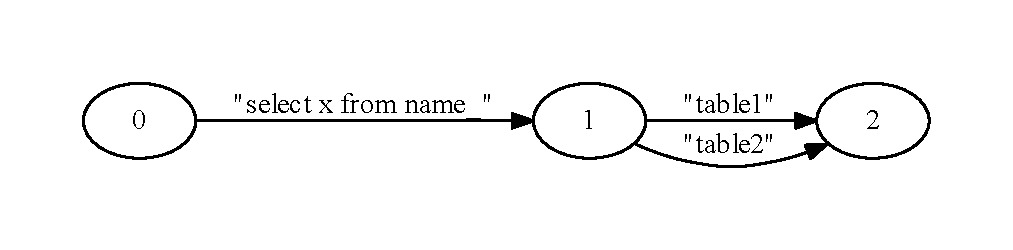
\includegraphics[width=\textwidth]{Polubelova/example_break}
\caption{Пример случая с ``рваными'' токенами}
\label{fig:example_break} 
\end{figure}

\item Осуществить корректную передачу координат токена в ReSharper.
\item Сравнить полученный инструмент с его аналогами.
\end{itemize}

\section{Обзор}
Для работы с динамически формируемыми строками существует ряд инструментов, основные особенности которых представлены ниже. 
Последние три инструмента интересны тем, что они имеют абстрактный анализ --- на вход подается компактное представление множества 
динамически формируемого выражения. Это может быть data-flow уравнение, регулярное выражение или граф. Первые два инструмента отвечают 
на вопрос --- является ли обрабатываемый язык подмножеством какого-нибудь языка. 
\begin{itemize}
\item \textbf{PHP string analyzer}\footnote{http://www.score.cs.tsukuba.ac.jp/~minamide/phpsa} --- это статический анализатор для строк, порождаемых программами на PHP. Он аппроксимирует значения 
таких строк некоторой контексно-свободной грамматикой.
\item \textbf{Java String Analyzer}\footnote{http://www.brics.dk/JSA} --- это инструмент для анализа формирования строк и строковых операций в программах на Java. 
Для каждого строкового выражения он строит конечный автомат, представляющий приближенное значение всех значений этого выражения, 
которые могут быть получены во время выполнения.
\item \textbf{Alvor} --- это плагин к среде разработки Eclipse, предназначенный для статической валидации SQL-выражений встроенных в код на Java. 
Найденные в коде  SQL-запросы проверяются на основе SQL-грамматики.  Компактным представлением множества динамически формируемых выражений для лексера 
является регулярное выражение.
\item \textbf{статья Kyung-Goo Doh, Hyunha Kim, David A. Schmidt}~\cite{Doh} --- предложили алгоритм абстрактного анализа на примере статической 
валидации  динамически генерируемого HTML в PHP. Абстрактный парсер на вход принимает data-flow уравнение и LALR(1) -- таблицу, в качестве результата 
выдает абстрактное синтаксическое дерево, пригодное для дальнейшего анализа. Парсер работает на символах, не на токенах. 
\item \textbf{инструмент YaccConstructor}\footnote{https://code.google.com/p/recursive-ascent} --- модульный инструмент для проведения лексического  
анализа и синтаксического разбора. Также является платформой для исследования и разработки генераторов абстрактных лексических и синтаксических анализаторов.
Структура инструмента представлена на рис.~\ref{fig:YC_base}

\begin{figure}[t]
\centering
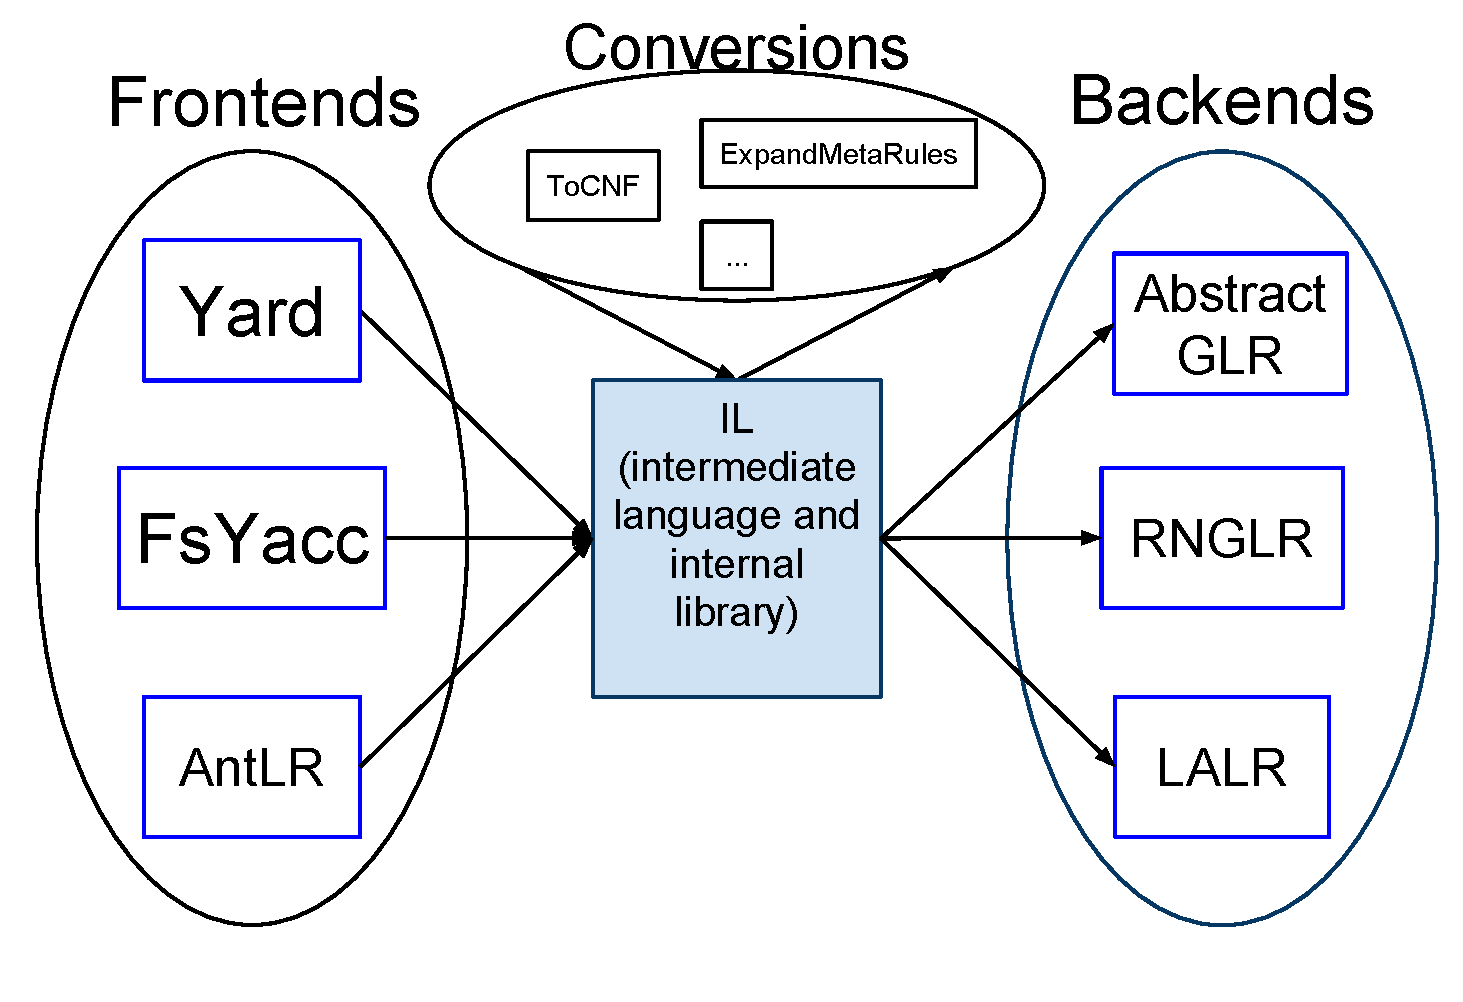
\includegraphics[width=\textwidth]{Polubelova/YC_base}
\caption{Структура инструмента YaccConstructor}
\label{fig:YC_base} 
\end{figure}


В рамках проекта YaccConstructor разрабатывается платформа для поддержки встроенных языков. Демонстрация возможностей разрабатываемой платформы представлена в виде плагина к ReSharper. Например, с помощью него можно подсвечивать ошибки (рис.~\ref{fig:ReSharper}) в Microsoft Visual Studio IDE. Для того чтобы это сделать, необходимы координаты токена в исходном коде, которые можно получить, сохранив привязку частей динамически формируемого выражения к исходному коду и привязку лексических единиц внутри каждой части при проведении абстрактного лексического анализа.

\begin{figure}[t]
\centering
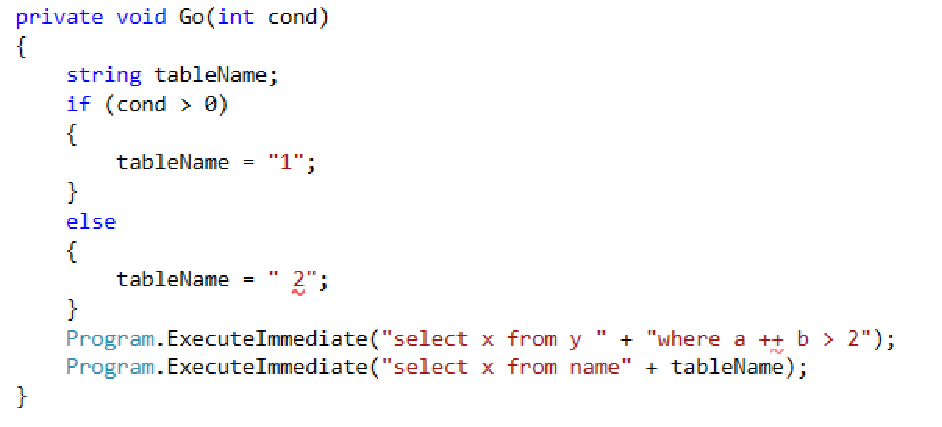
\includegraphics[width=\textwidth]{Polubelova/ReSharper}
\caption{Подсветка ошибок в Microsoft Visual Studio IDE}
\label{fig:ReSharper} 
\end{figure}
\end{itemize}


\section{Реализация}

%\begin{enumerate}

\subsection {Генератор абстрактных лексических анализаторов}

В рамках проекта YaccConstructor был реализован генератор абстрактных лексических анализаторов, который по спецификации генерирует лексический 
анализатор для обрабатываемого языка. В качестве основы для него был взят генератор лексических анализаторов для F\# --- FsLex. 
Структура генератора представлена на рис.~\ref{fig:Generator}

\begin{figure}[t]
\centering
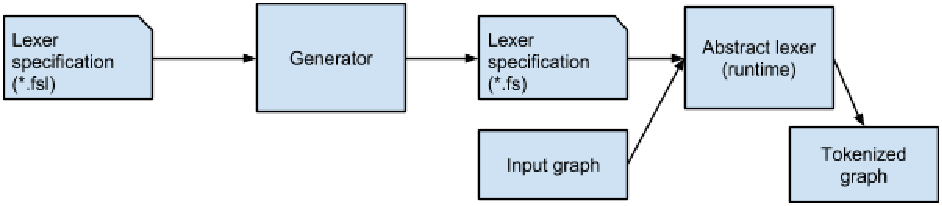
\includegraphics[width=\textwidth]{Polubelova/Generator}
\caption{Структура генератора в YaccConstructor}
\label{fig:Generator} 
\end{figure}

Входной структурой для анализатора является граф --- компактное представление множества динамически формируемых выражений, которые могут быть получены 
посредством конкатенации строковых констант и выражений встроенного языка в цикле, условных выражениях и другими способами. Ограничения на граф --- граф 
является DAG-ом (направленный ациклический граф), у которого одна стартовая и одна конечная вершина. Для конечной вершины верно, что из нее не выходит ни 
одна дуга. Это достигается явным добавлением дуги с токеном, обозначающим конец ввода. Абстрактный лексический анализатор основан на конечном преобразователе. 
Это конечный автомат, который может выводить конечное число символов для каждого входного символа. На основе него лексер переводит входной граф в граф, 
содержащий соответствующие спецификации токены. 

Результат аппроксимации динамически формируемых выражений, представленных на рис.~\ref{fig:ReSharper}, можно увидеть на рис.~\ref{fig:Graph1} и рис.~\ref{fig:Graph2}.
	
\begin{figure}[t]
\centering
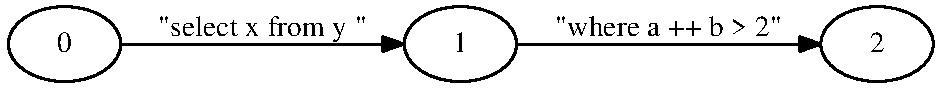
\includegraphics[width=\textwidth]{Polubelova/Graph1}
\caption{Граф для первого запроса}
\label{fig:Graph1} 
\end{figure}

\begin{figure}[t]
\centering
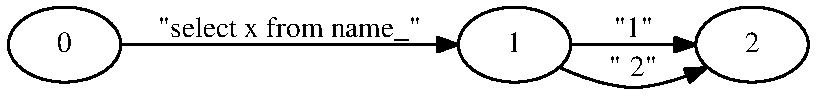
\includegraphics[width=\textwidth]{Polubelova/Graph2}
\caption{Граф для второго запроса}
\label{fig:Graph2} 
\end{figure}

Поскольку динамически формируемые выражения могут быть получены с помощью конкатенации строковых констант и выражений встроенного языка в цикле, 
условных выражениях и другими способами, то возникают ситуации с ``рваными'' токенами. В реализованном инструменте был предложен следующий алгоритм 
для обработки таких случаев:

\begin{enumerate}
\item	На вход подаётся граф, составленный на основе дерева разбора исходного кода программы: на ребрах — фрагменты строк кода на встроенном языке, 
вершинам соответствуют случаи конкатенации строк.
\item	Входной граф преобразовывается к виду, удобному для лексического анализа: каждое ребро входного графа разбивается на последовательность новых 
ребер, метки которых содержат не более одного символа из строки исходного ребра.
\item   Запускается процедура токенизации на преобразованном графе, заключающаяся в вычислении множества возможных состояний лексического анализатора
в каждой вершине входного графа. В случае, если в какой-либо вершине получено финальное состояние, то из накопленной строки формируется токен согласно 
соответствующему пользовательскому коду, и в множество состояний для данной вершины заносится стартовое состояние. В результате данной процедуры получается
новый граф, на ребрах которого находятся накопленные в результате работы токены, соответствующие грамматике анализируемого встроенного языка
\end{enumerate}

На рис.~\ref{fig:example_calc_break} представлен пример входного графа с ``разрывными'' токенами. Результат работы абстрактного лексического 
анализатора над этим графом показан на рис.~\ref{fig:res_ex_calc_break}

\begin{figure}[t]
\centering
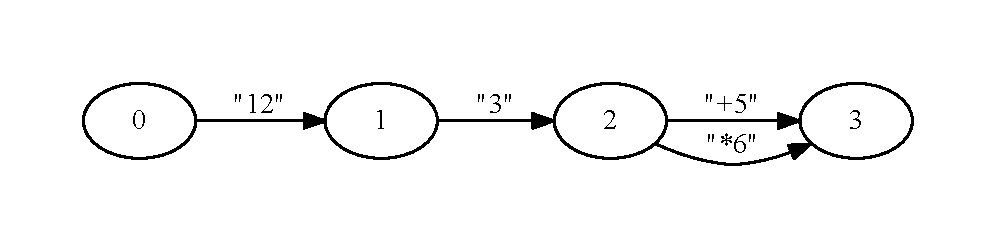
\includegraphics[width=\textwidth]{Polubelova/example_calc_break}
\caption{Пример графа с ``разрывными'' токенами }
\label{fig:example_calc_break} 
\end{figure}

\begin{figure}[t]
\centering
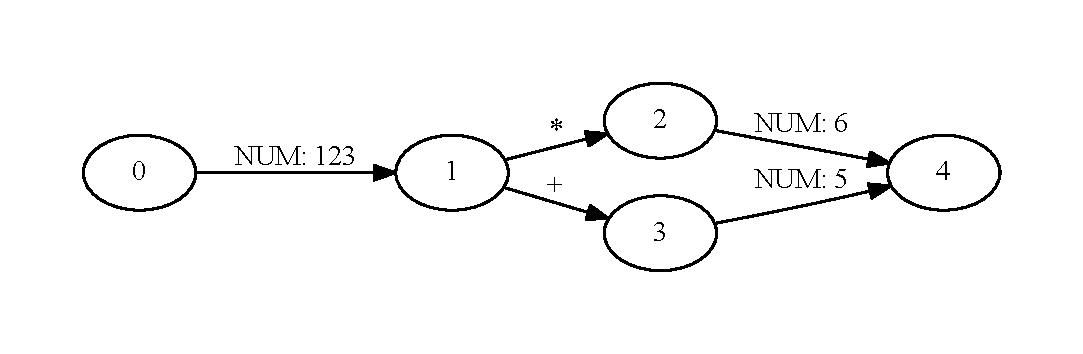
\includegraphics[width=\textwidth]{Polubelova/res_ex_calc_break}
\caption{Результат работы лексера в случаи ``разрывных'' токенов }
\label{fig:res_ex_calc_break} 
\end{figure}

Существующий генератор абстрактных лексических анализаторов был модифицирован таким образом, чтобы он умел корректно обрабатывать случаи, 
когда на дугах входного графа находятся пробелы и комментарии. В связи с этим добавился этап построения eps-замыкания токенизированного графа.
Пример такого графа представлен на рис.~\ref{fig:example_space}. Результат работы лексера представлен на рис.~\ref{fig:res_ex_space}.

\begin{figure}[t]
\centering
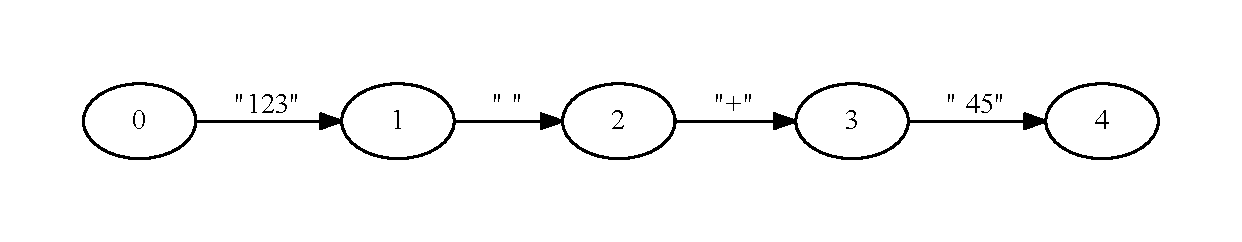
\includegraphics[width=\textwidth]{Polubelova/example_space}
\caption{Пример графа, на ребрах которого находятся пробелы}
\label{fig:example_space} 
\end{figure}

\begin{figure}[t]
\centering
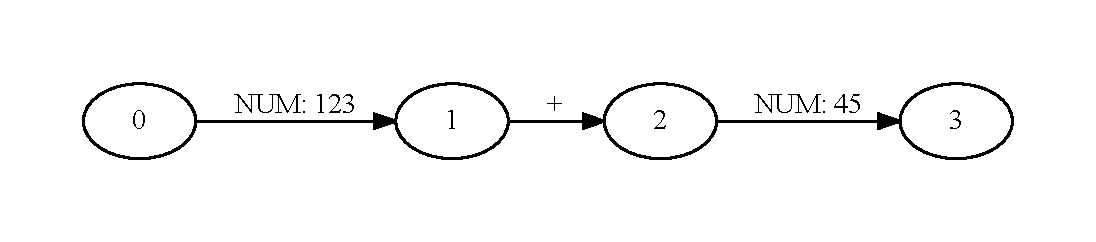
\includegraphics[width=\textwidth]{Polubelova/res_ex_space}
\caption{Результат работы лексера, когда ребра входного графа содержали пробелы}
\label{fig:res_ex_space} 
\end{figure}

Также в ходе разбора входных данных абстрактный лексический анализатор сохраняет привязку частей динамически формируемого выражения к исходному коду и 
привязку лексических единиц внутри каждой части. Для этого к существующей структуре, которая хранила информацию о токене, было добавлено новое поле Positions.
Оно хранит для каждого символа токена строку из которой он получен и позицию этого символа внутри этой строки.  Для корректного вычисления позиции токена в
случае ``рваных'' токенов была добавлена глобальная структура LexBuffer, которая хранит состояние графа после каждого прочитанного символа. 

Результат работы абстрактного лексического анализатора с сохранением привязки к исходному коду показан на рис.~\ref{fig:res_ex_calc_bounded}, где входной структурой являлся граф, представленный на рис.~\ref{fig:res_ex_calc_break} 

\begin{figure}[t]
\centering
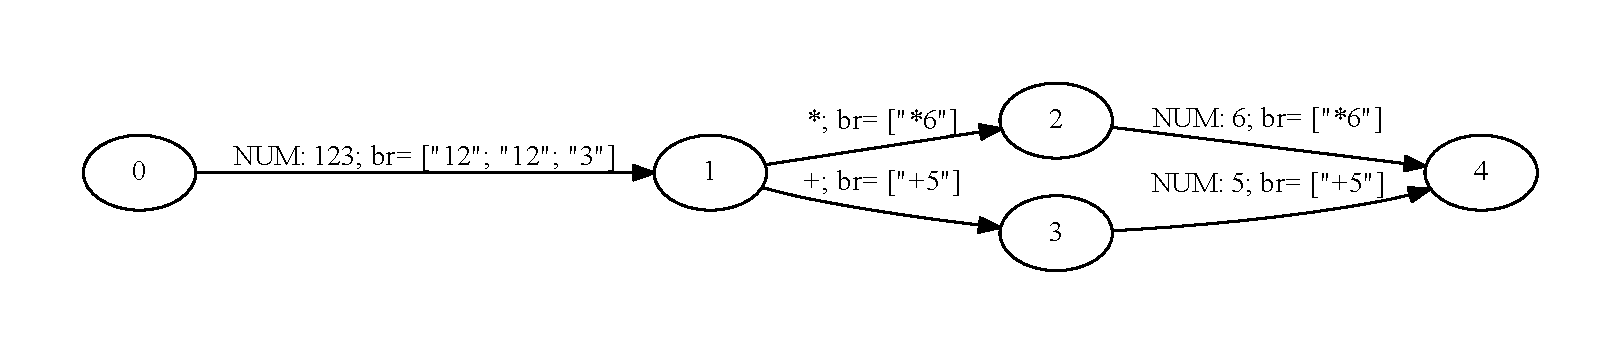
\includegraphics[width=\linewidth]{Polubelova/res_ex_calc_bounded}
\caption{Результат работы лексера с сохранением привязки к исходному коду}
\label{fig:res_ex_calc_bounded} 
\end{figure}	


Одним из примеров использования данной привязки является позиционирование токена в исходном коде, поскольку она позволяет однозначным образом определить
в какой строке и на какой позиции внутри этой строки находится токен. Это нужно, например, для подсветки синтаксиса.

\subsection {Инструмент для тестирования лексера инструментов YaccConstructor и Alvor}

В обзоре был представлен ряд инструментов, которые работают с динамически формируемыми выражениями. Поскольку только инструмент Alvor решает схожую 
задачу с инструментом YaccConstructor и имеет открытые исходники, то сравнение происходило только с ним.  В инструменте Alvor, так же как и в YaccConstructor, 
отдельно выделены этапы лексического анализа и синтаксического разбора. Входными данными для лексера Alvor является регулярное выражение --- компактное представление 
множества значений динамически формируемого выражения. 

В рамках данной работы был реализован генератор тестов, который по двум заданным параметрам $m$(кратность ребер) и $n$(длина цепочки) выдает граф в формате .dot, генератор замеров времени работы лексера YaccConstructor и Alvor, генератор тестов, который переводит данные, представленные в формате .dot, в регулярное выражение, записанного потом в текстовый файл. 

Пример  графа, который может быть получен с помощью генератора тестов в формате .dot с параметрами $m~=~2$ и $n~=~3$, представлен на рис.~\ref{fig:m2_n3} (a и b используются в качестве ограничителя). Для лексера Alvor данный граф запишется в следующее регулярное выражение, которое можно увидеть 
на рис.~\ref{fig:m2_n3_alvor}. 
 
\begin{figure}[t]
\centering
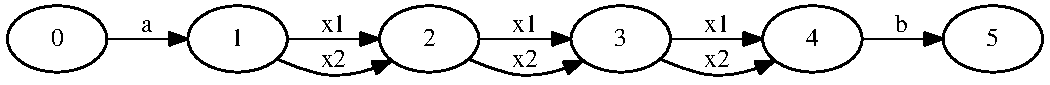
\includegraphics[width=\textwidth]{Polubelova/m2_n3}
\caption{Пример графа с параметрами $m = 2$ и $n = 3$}
\label{fig:m2_n3} 
\end{figure}

\begin{figure}[t]
\centering
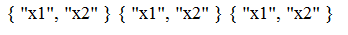
\includegraphics[width=0.5\textwidth]{Polubelova/m2_n3_alvor}
\caption{Пример регулярного выражения с параметрами $m = 2$ и $n = 3$}
\label{fig:m2_n3_alvor} 
\end{figure}

Компоненты реализованного инструмента можно использовать независимо друг от друга. Например, для лексера в качестве входных данных можно использовать тесты, 
которые были получены другим генератором тестов.  Полученные результаты замеров работы лексера можно визуализировать с помощью R-studio с целью получения графика, 
например, зависимости времени от сложности лексического разбора входных данных. Для визуализации файлов с расширением .dot можно использовать Graphviz.

%\end{enumerate}
\begin{figure}[ht]
        \centering
        \subfloat[с ``разрывными'' токенами]{
                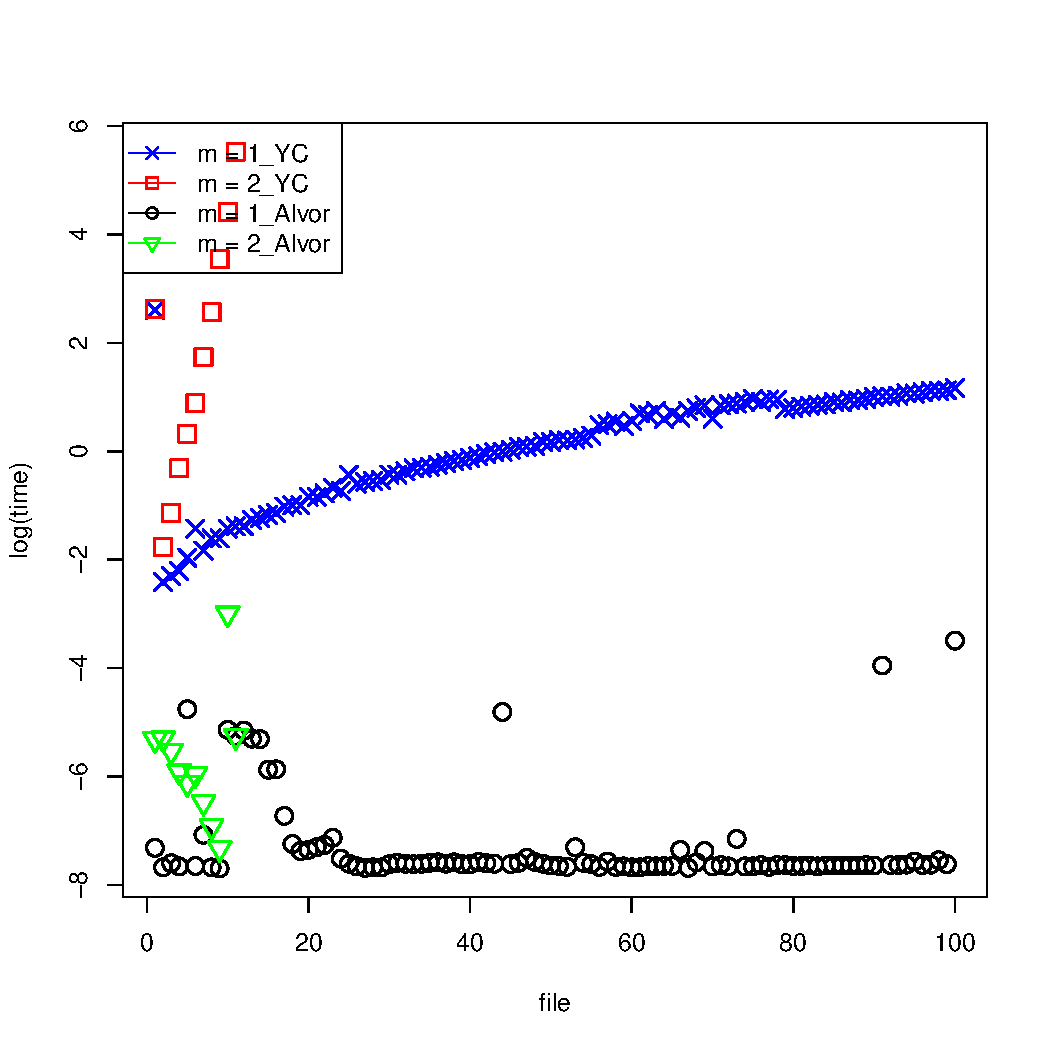
\includegraphics[width=0.7\textwidth]{Polubelova/YC_Alvor_break}
                %\caption{с ``разрывными'' токенами}
                \label{fig:YC_withBreak}
        }\\
         %add desired spacing between images, e. g. ~, \quad, \qquad, \hfill etc.
          %(or a blank line to force the subfigure onto a new line)
        \subfloat[с неразрывными токенами]{
                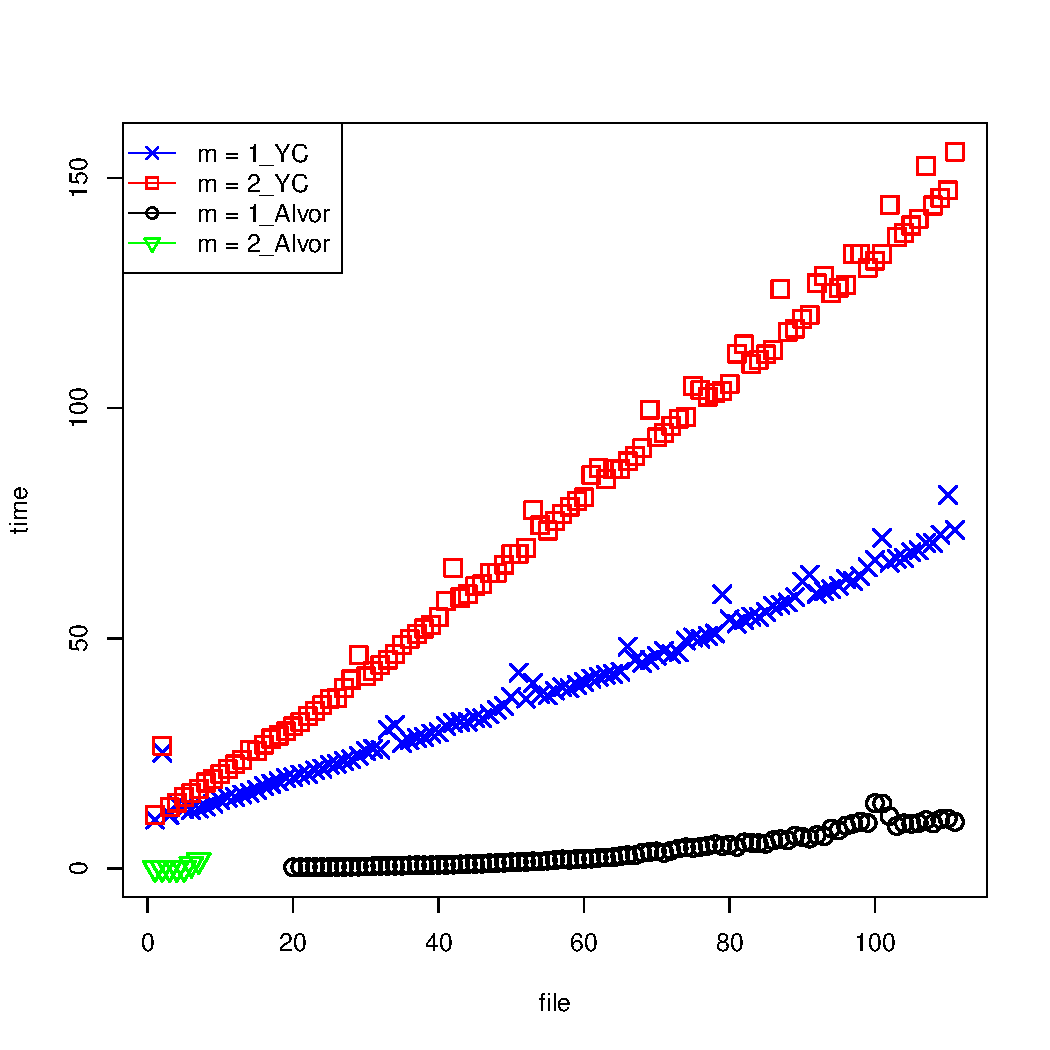
\includegraphics[width=0.7\textwidth]{Polubelova/YC_Alvor}
                %\caption{с неразрывными токенами}
                \label{fig:YC_withoutBreak}
        }
        \caption{Графики для YC и Alvor}\label{fig:graphs_yc_alvor}
\end{figure}
\clearpage

\section{Апробация}
Большинство  программ, написанные на SQL, содержат в себе вложенные конструкции языка, которые формируются с помощью условных выражений, конкатенаций и другими строковыми операциями. 
Для анализа программы необходимо рассмотреть все возможные случаи, которые могут получиться из динамически формируемого выражения. Поэтому для тестирования работы абстрактного лексического анализатора были выбраны тесты, которые описаны в пункте ``Инструмент для тестирования лексера инструментов YaccConstructor и Alvor''.

Так как во встроенных языках возможны случаи с ``разрывными'' токенами --- когда токен находился на двух и более ребрах исходного графа, то были подобраны тесты и 
с ``разрывными'' токенами. Разумным считается, что длина цепочки не может быть большой --- на практике редко встретишь, чтобы идентификатор был составлен при помощи
большого числа конкатенаций. Структура теста такая же как в случаи безразрывных токенов. 

В обзоре был представлен ряд инструментов, которые работают с динамически формируемыми выражениями. Сравнение времени работы лексера было проведено
для инструментов YaccConstructor и Alvor. Замеры времени работы лексера указанных инструментов проводились на машине со следующими техническими характеристиками:
Intel(R) Core(TM) i7-3537U CPU @ 2.00GHz 2.50 GHz, 4,00 Гб оперативной памяти, процессор x64.

Были рассмотрены случаи с безразрывными токенами для m = 1, 2, 5 и n~=~8..228 с шагом 2. Лексер инструмента Alvor разбирает данные быстрее, чем лексер инструмента YaccConstructr, но Alvor не обрабатывает случаи, когда на вход ему 
было подано регулярное выражение, содержащее большое количество альтернатив, в то  время как YC аналогичные данные, только представленные 
в виде графа,  обработал. 

Также были рассмотрены случаи с ``разрывными'' токенами для m = 1, 2, 5 и n~=~1..100.
Также лексер инструмента Alvor обработал входные данные быстрее, чем лексер инструмента YaccConstructor. Длина цепочки входного графа, которую разбирают лексеры этих инструментов, примерно одинаковая. 
На больших значениях параметоров m и n графа, лексеры инструментов завершают работу с ошибкой о переполнении стека. 

На рис.~\ref{fig:graphs_yc_alvor} можно увидеть график, 
на котором показаны результаты замеров работы лексера инструментов YaccConstructor и Alvor. 
Видно, что время разбора лексера увеличивается от сложности входных данных. В случае обычных литералов для инструмента YC почти линейно, а в случае 
``разрывных'' токенов экспоненциально. Для инструмента Alvor для обычных токенов экспоненциально, поскольку они перебирают все варианты и возвращают 
только уникальные результаты лексического разбора. 

% У заключения нет номера главы
\section*{Заключение}
В ходе выполнения данной работы были получены следующие результаты:
\begin{itemize}
\item Реализовано сохранение привязки частей динамически формируемого выражения к исходному коду и привязки лексических единиц внутри каждой части.
\item Осуществлена корректная передача координат токена в ReSharper.
\item Доработан генератор абстрактных лексических анализаторов так, чтобы он корректно обрабатывал комментарии и пробелы.
\item Изучены аналоги лексических анализаторов.
\item Реализован инструмент для тестирования лексеров YaccConstructor и Alvor.
\item Проведен анализ времени работы генераторов YaccConstructor и Alvor на одинаковых входных данных.
\end{itemize}

На практике не каждый случай использования встроенных языков может быть представлен в виде направленного ациклического графа. 
В дальнейшем хочется научиться поддерживать графы, содержащие циклы. Также планируется в инструменте YaccConstructor реализовать 
конечный преобразователь~\cite{Mehryar}, который будет поддерживать строковые операции, например, replace.

\begin{thebibliography}{99}
\bibitem{YC_article}
Я.А.Кириленко, С.В.Григорьев, Д.А.Авдюхин.
Разработка синтаксических анализаторов в проектах по автоматизированному реинжинирингу информационных систем //
Научно-технические ведомости Санкт-Петербургского государственного политехнического университета. Информатика. Телекоммуникации. Управление.
\No 174, 2013.

\bibitem{Doh}
Kyung-Goo Doh, Hyunha Kim, David A. Schmidt.
Abstract LR-Parsing // Formal Modeling: Actors, Open Systems, Biological Systems, 2011.

\bibitem{Annamaa}
Aivar Annamaa, Andrey Breslav, Varmo Vene.
Using Abstract Lexical Analysis and Parsing to Detect Errors in String-Embedded DSL Statement //
Proceedings of the 22nd Nordic Workshop on Programming Theory, 2010.

\bibitem{Breslav}
Andrey Breslav. Parsing Abstract Strings. University of Tartu, 2010.

\bibitem{Mehryar}
Mohri Mehryar. Finite-State Transducers in Language and Speech Processing. Association for Computational Linguistics, 
1997.
\end{thebibliography}
